\begin{figure}[H]
	\centering
	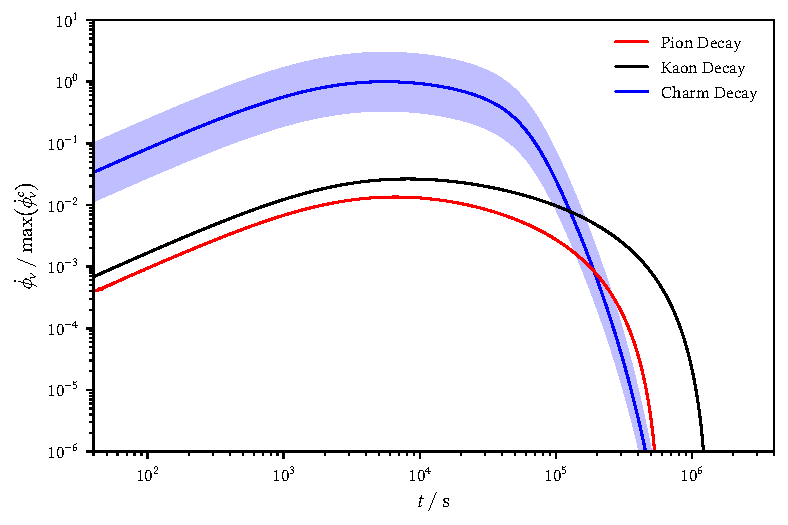
\includegraphics{../plots/build/magnetar_neutrino_spectrum_with.pdf}
	\caption[Magnetar $\nu \kern+0.5pt$ flux compared to $c$ decay with optical depth.]
			{Effective neutrino light curves normalized to the maximum charm decay flux at
			 $E_\nu = \kern-0.5pt \qty{e9}{\giga\electronvolt}$ from a newborn magnetar, including the optical depth
			 defined by \eqref{eqn:optical} as a modification. Charmed hadrons dominate up to $t = \kern-0.5pt \qty{e5}{\second}$
			 with pion contributions below those from kaons at all times. A cutoff after $t = \kern-0.5pt \qty{e6}{\second}$ occurs
			 due to insufficient proton energies. For the charm component, a shaded blue error band with a width factor ranging from
			 $1 \kern-0.5pt /3$ to $3$ is adopted to replicate the uncertainties from \cite{Carpio_2020}.}
	\label{fig:magnetar-flux-with}
\end{figure}
